\documentclass[10pt,twocolumn,letterpaper]{article}

\usepackage{cvpr}
\usepackage{times}
\usepackage{epsfig}
\usepackage{graphicx}
\usepackage{amsmath}
\usepackage{amssymb}

\usepackage{paralist}


% Include other packages here, before hyperref.

% If you comment hyperref and then uncomment it, you should delete
% egpaper.aux before re-running latex.  (Or just hit 'q' on the first latex
% run, let it finish, and you should be clear).
\usepackage[breaklinks=true,bookmarks=false]{hyperref}

\cvprfinalcopy % *** Uncomment this line for the final submission

\def\cvprPaperID{****} % *** Enter the CVPR Paper ID here
\def\httilde{\mbox{\tt\raisebox{-.5ex}{\symbol{126}}}}

% Pages are numbered in submission mode, and unnumbered in camera-ready
%\ifcvprfinal\pagestyle{empty}\fi
\setcounter{page}{4321}
\begin{document}

%%%%%%%%% TITLE
\title{Semantic Labeling of Images Using SVM Classifiers}

\author{Daniel McArdle\\
University at Buffalo\\
Buffalo, NY\\
{\tt\small demcardl@buffalo.edu}
}

\maketitle
%\thispagestyle{empty}

%%%%%%%%% BODY TEXT
\section{Introduction}

Holistic scene understanding is an open problem in the area of Computer Vision.  However, smaller subsets of this large problem are easier to approximate a solution for.  These application-specific subsets can be used for autonomous vehicles, robotics, semantic analysis for image search, and video surveillance or crowd statistics, to name a few.

In this project, the subset we aim to solve is superpixel-level semantic labeling using SVMs for eight classes: Sky, Tree, Road, Grass, Water, Building, Mountains, and Foreground.  Specifically, we are trying to optimize the quality of results of the given superpixel classifier. Since there are eight classes, there are eight separate SVMs. Each SVM probabilistically determines class membership for a single class.

While attempting different changes and measuring their effects on performance, multiple SVM kernel filters were evaluated, as well as two different types of features.  The types of kernel filters evaluated were as follows: linear (the default), Gaussian, and 3rd- and 5th-degree polynomials. The first new feature evaluated was a scaled $(x,y)$ coordinate feature, rather than the given histogram of all pixels' $y$ values. The second new feature evaluated was SIFT features, computed for each superpixel.

\section{Related Work}




\subsection{A Scene Classification Method Based on Ensemble SVM Results \cite{luo}}
\label{sec:luo_section}

The method proposed by this paper is broken into two phases: training and testing. The training phase makes use of SIFT features, visual vocabularies, Bag-of-Words models, and latent semantic features in order to separately train $n$ different SVM classifiers.  In testing, all $n$ SVMs are used to classify the testing images.

The method also uses Probablistic Latent Semantic Analysis (PLSA), a technique originally used in the domain of Natural Language Processing.  PLSA is the joint probability of the vocabulary and the document.  This process computes a $T$-dimensional vector that defines an image's latent semantic features.

This paper is quite similar to our project's general structure.  Their use of Bag-of-Words using SIFT features with K-Means clustering has been incorporated into our project.  We are performing K-Means clustering on the SIFT features of each superpixel and adding those $k$ features to the feature vector for the superpixel.


\subsection{Recovering Surface Layout from an Image \cite{hoiem}}

This paper begins by discussing humans' innate skill for reconstruction of a 3D scene from a 2D input, such as a photograph.  After discussing theories of human vision, they briefly review early failed attempts at computer vision algorithms.

The paper's focus is labeling coarse geometric classes of outdoor scenes. These classes could be used for navigation, object recognition, and general scene understanding.

The main insight of this paper is that, according to their experimental results from outdoor images obtained with Google image search, 97\% of all pixels belong to one of three classes: horizontal (support) surfaces, vertical surfaces, or the sky.   Unsurprisingly, the three geometric classes they chose are named "horizontal," "vertical," and "sky."

To determine the orientation of the surface generating a patch in the 2D image, their algorithm relies on multiple cues: location, color, texture, and perspective.

This paper suggests use of local features that we are already using.  We are including location, color, and texture in our feature vector. It would be useful if we could include perspective information. This might be done with vanishing point or parallel line detection, but it was not included in our experiment.

\subsection{Decomposing a Scene into Geometric and Semantically Consistent Regions \cite{gould}}

Superpixels' boundaries are often inconsistent with the true segment boundaries because they are constructed using only local appearance information.  

This paper's approach is to create regions that should correspond to a complete segment, but have dynamic boundaries. This allows more than global features to be used, including shape, aspect ratio, and boundary characteristics.

Many prior algorithms optimize region appearance, class labels, etc. in separate stages. In contrast to this prior work, this paper features a holistic energy function that simultaneously optimizes the pixel-to-region associations, the region semantic class labels, geometries, and appearances, as well as the horizon location.

The technique of using dynamic region boundaries was not adopted for our project. Superpixels formed from local features were used instead of dynamic regions.  Despite that, the paper features a novel, but different, approach the same problem we are trying to solve.

\subsection{Learning Multi-Label Scene Classification \cite{Boutell20041757}}

Boutell posits that it is useful to reevaluate the assumption that classes are mutually exclusive by definition. This assumption causes avoidable classification errors to occur.  Sometimes, it is the case that data really does belong to multiple classes.

The author speaks about prior attempts at multiple class membership.  It is important to see the distinction between a scene being a fuzzy member of two classes (a symptom of ambiguity) and being a complete member of two classes (both classes are completely and equally applicable).

Our project is firmly rooted with the assumption that classes are mutually exclusive.  
The assumption of mutually-exclusive classes is made during the testing phase, when we select the maximum response from the $n$ trained SVMs. Unfortunately, this paper's approach is too different to borrow any techniques.  

\subsection{Multiple View Semantic Segmentation for Street View Images \cite{xiao}}

This paper describes an algorithm that uses Markov Random Fields on Google Street View images.  The nature of the data set is that there are multiple photos of the same object taken from different views, as the car the camera is mounted on drives past.  These researchers took advantage of that fact to improve performance.

Structure from Motion is used to recreate the 3D scene from a series of 2D photos.  The MRF is laid out across the sequence of relevant images.  A novel 3D user-labeling approach is proposed for saving time on generating ground-truth data.

This paper does not use SVMs and it does not have many borrowable techniques.  It shows some options, however, when dealing with a different problem domain than we are. Specifically, if we had more data from different angles, different techniques would become more feasible, such as MRF.

\subsection{An Ontology for Generating Descriptions about Natural Outdoor Scenes \cite{nwogu}}

This paper describes an system that uses an new ontology, with predefined constructs for relevant content, in order to generate English sentences accurately describing a single scene.  It shows a novel algorithm combining the fields of Knowledge Representation and Computer Vision.

The segmentation algorithm uses uses a graph where nodes represent superpixels and edges represent the fact that two superpixels are touching.  Image gradient magnitudes are given to an implementation of the watershed segmentation algorithm.  Then, some of these superpixels are merged together, using a threshold value and the $\chi^2$ similarity of the superpixel feature vectors.  Using the GIST descriptors for an image, a one-versus-all test is performed with an SVM (this is a class inclusion test, the normal mode of operation for a SVM).

After the segmentation, spatial, color shape, and texture features, as well as holistic features such as vanishing points, estimated horizon, and percentage of nearly-parallel lines are used to identify the class of object (possible choices are people, cars, trains, motorbikes, buses, cows and boats).

In the end, the descriptive natural-language sentences are generated using enhanced templates and production rules, which are more powerful than slot-filling sentence generation.

The approach for segmentation and recognition in this paper is the most applicable to our project.  The easiest idea to borrow would be using local features from GIST, rather than SIFT, to add more data to the superpixel feature vectors.  Their segmentation algorithm takes advantage of spatial proximity of superpixels, specifically when performing superpixel merging, but ours treats each superpixel independently.  The segmentation algorithm would be a valuable technique to incorporate.

\section{Approach}

The algorithm is broken up into three parts: \begin{inparaenum}
\item Feature extraction, \item Training, and \item Testing
\end{inparaenum}.

In order to generate results in a reasonable amount of time, two "debug" parameters have been introduced to the code.
\begin{enumerate}
\item The first is \texttt{SP\_SUBSET}, short for "superpixel subset." This value controls the number of superpixels fed to the SVM during training mode.
\item The second is \texttt{IM\_SUBSET}, short for "image subset." This value restricts the number of images used in the feature extraction process.
\end{enumerate}

\subsection{Feature Extraction}

For each superpixel in each image, many types of local features are encoded in a feature vector.  These features are RGB, HSV, mean texture response, max texture response, a histogram of the y values, and SIFT features.

The RGB value is computed as the mean pixel value for all the pixels in the subset. Then, the HSV value is simply the equivalent color in the HSV color space.

The mean and max texture response are computed with the \texttt{imtext} function.

The histogram of $y$ values of a pixel is potentially helpful for discriminating between the "Sky" class and other classes. The closer a pixel is to the top of the image, the more likely that it is a member of the Sky class.

\subsubsection{SIFT Features}

SIFT features are computed using the MATLAB library VLFeat \cite{vlfeat}.  The SIFT features for each superpixel are computed as part of the same loop discussed above.

After computing the SIFT features, they are clustered using K-Means, with $k=3$.  This treatment of SIFT features was recommended by "A Scene Classification Method Based on Ensemble SVM Results" \cite{luo}, discussed above in section ~\ref{sec:luo_section}.

It is important to note that not every superpixel has $k$ SIFT features in it; in fact, some have zero.  In these cases, where $m<k$ and $m$ is the actual number of SIFT features in the superpixel, we simply add $k-m$ zero-valued features.  This consistency check is so that we always have a constant-length feature vector across all superpixels.

\subsection{Training/Testing}

Training is performed in \texttt{trainSceneLabels}.  The procedure is to take the superpixel features that were extracted in the previous step, the ground-truth superpixel labels, and feed them to $n$ different SVMs (one for each class) using \texttt{fitcsvm} with a linear kernel.

During testing, the selected test feature vectors are fed to each of the $n$ SVMs created in the previous step. The SVM with the maximum response is selected and its corresponding class is then the class of the given superpixel.

At the end of testing, a confusion matrix is computed using the ground-truth data, where the value at $(i,j)$ represents the percent of real class-$i$ images classified as class-$j$.  The mean of the confusion matrix's diagonal gives the average percent of correctly-classified superpixels.

\subsection{Abandoned Changes}

Different SVM kernels and an $(x,y)$ coordinate feature (in lieu of the $y$ histogram) were tested. Experimentally, these were determined to have worse performance than the baseline code, and the changes were reverted.

In the interest of time, these changes were only tested for fold \#4, but with 50,000 superpixels. Since the tests were performed on only a single fold, the results below should not be considered conclusive.

Future testing with more superpixels and Five-Fold Cross Validation could determine the optimal choice of kernel function.

\subsubsection{SVM Kernel Results}

\begin{center}
  \begin{tabular}{ l | l }
  	\textbf{Kernel} & \textbf{Performance (\%)}\\
    \hline
    Linear (default) & 14.1419 \\ \hline
    Gaussian & 12.9358 \\ \hline
    3rd-Degree Polynomial & 13.5537  \\ \hline
    5th-Degree Polynomial & 13.8650  \\
    \hline
  \end{tabular}
\end{center}

\subsubsection{Other Features}
Additionally, a version of the code where the $y$-value histogram in the feature vector was replaced with the average $x$ and $y$ coordinates was examined.  The performance for this attempt was 12.4451\%, which was worse than the baseline 14.1419\%.

\section{Experimental Analysis and Results}

The 5-Fold Cross-Validation was performed once, for 10,000 superpixels, the results of which can be seen below in section ~\ref{sec:crossVal}.  This was accomplished by making \texttt{fold\_idx} take on the values of one through five in \texttt{trainSceneLabels.m} and \texttt{testSceneLabels.m} and then running the two functions in succession after each change.

The only change between the baseline and the new version of the code is that K-Means-clustered SIFT features were added.  Comparing the means, it appears that the SIFT features hurt the accuracy of the classifier.

Comparing the mean accuracy values for the baseline code with the version using SIFT, it would appear that the addition of SIFT features lowered accuracy.  However, we can see that the version with SIFT has a higher maximum accuracy as well as a higher minimum accuracy than the baseline.  It is simply the distribution of accuracy values across the folds that brings down the mean value.

To get a better answer on which version is more accurate, we would need to boost the number of superpixels to something much greater than 10,000. Ideally, we would test on all 316,824 superpixels in the dataset.  The fact that \begin{inparaenum} \item the accuracy of the baseline version did not approach the expected 50\% and \item that the class histograms (see figures 1-5) have many zero-valued classes \end{inparaenum} suggests that 10,000 superpixels is not enough for a fair comparison.

\subsection{5-Fold Cross-Validation for 10,000 Superpixels}
\label{sec:crossVal}

\begin{center}
  \begin{tabular}{ c | r | r }
  	\textbf{Fold \#} & \textbf{Baseline (\%)} & \textbf{With SIFT (\%)} \\
    \hline
    1 & 11.5025 & 10.9533\\ \hline
    2 & 13.2416 & 11.3602\\ \hline
    3 & 10.3480 & 10.9432\\ \hline
    4 & 13.5525 & 14.2296\\ \hline
    5 & 13.9880 & 11.7431\\ \hline
    -- & Mean: \hfill 12.5265 & Mean: \hfill 11.8459\\ \hline
    -- & Min: \hfill 10.3480 & Min: \hfill 10.9432\\ \hline
    -- & Max: \hfill 13.9880 & Max: \hfill 14.2296\\
    \hline
  \end{tabular}
\end{center}


% FOLD 1 RESULTS
\begin{figure}[p]
 \centering
 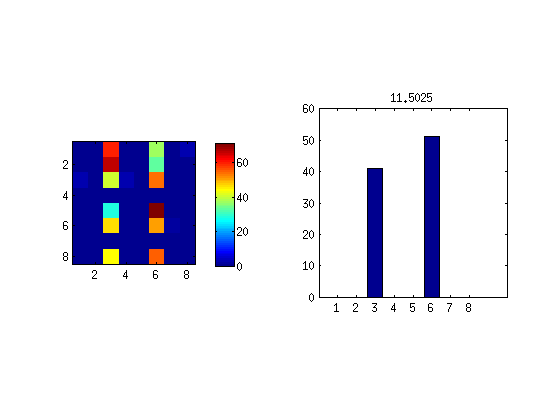
\includegraphics[scale=0.5]{../../../evaluation/baseline/fold1_1e5.png}
 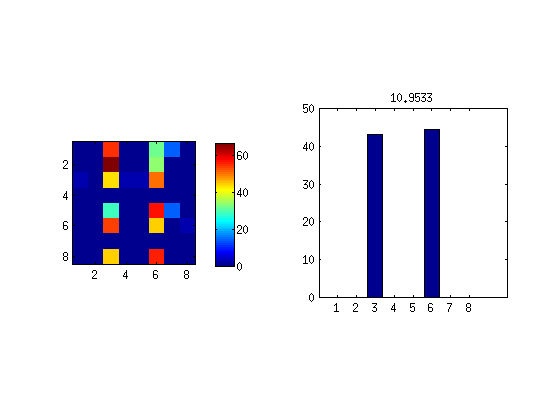
\includegraphics[scale=0.5]{../../../evaluation/feature-sift/fold1_1e5.png}
 \caption{Baseline Fold 1 (top); With SIFT Fold 1 (bottom)}
 \label{figure:withSiftFold1}
\end{figure}

% FOLD 2 RESULTS
\begin{figure}[p]
 \centering
 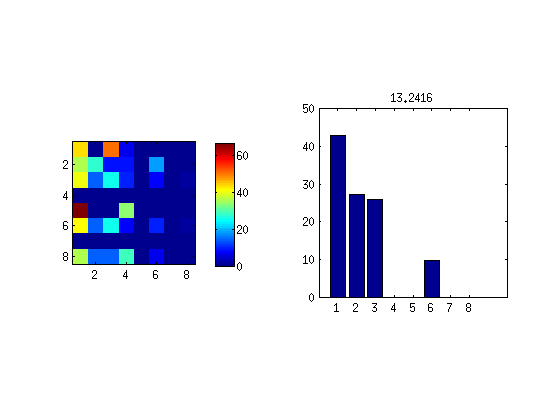
\includegraphics[scale=0.5]{../../../evaluation/baseline/fold2_1e5.png}
 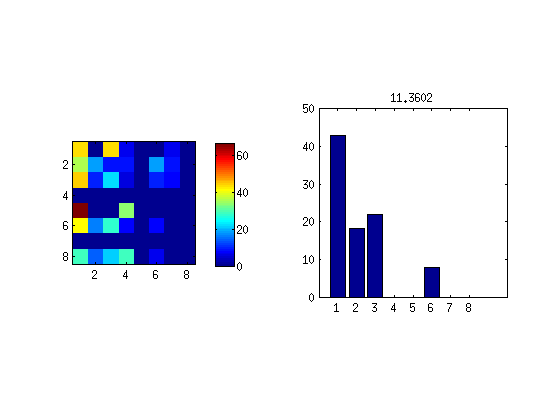
\includegraphics[scale=0.5]{../../../evaluation/feature-sift/fold2_1e5.png}
 \caption{Baseline Fold 2 (top); With SIFT Fold 2 (bottom)}
 \label{figure:withSiftFold2}
\end{figure}

% FOLD 3 RESULTS
\begin{figure}[p]
 \centering
 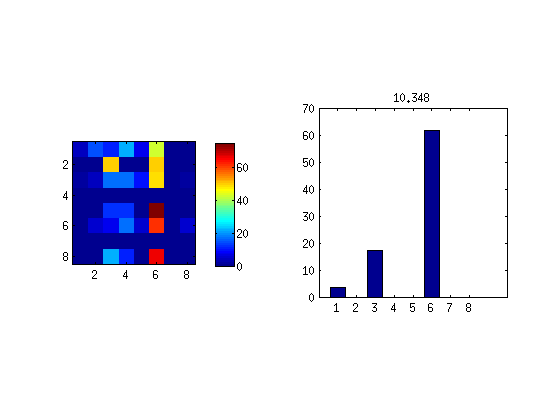
\includegraphics[scale=0.5]{../../../evaluation/baseline/fold3_1e5.png}
 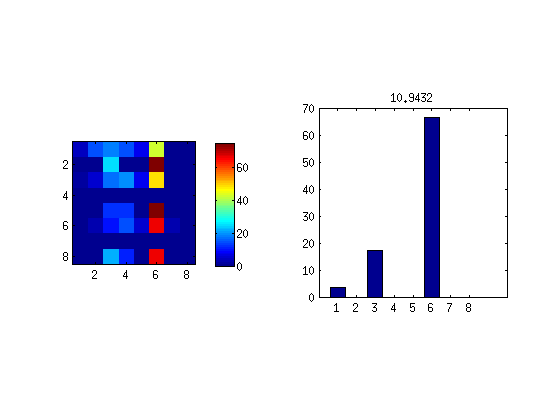
\includegraphics[scale=0.5]{../../../evaluation/feature-sift/fold3_1e5.png}
 \caption{Baseline Fold 3 (top); With SIFT Fold 3 (bottom)}
 \label{figure:withSiftFold3}
\end{figure}

% FOLD 4 RESULTS
\begin{figure}[p]
 \centering
 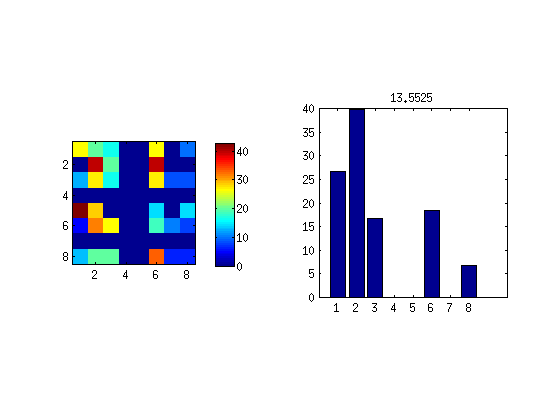
\includegraphics[scale=0.5]{../../../evaluation/baseline/fold4_1e5.png}
 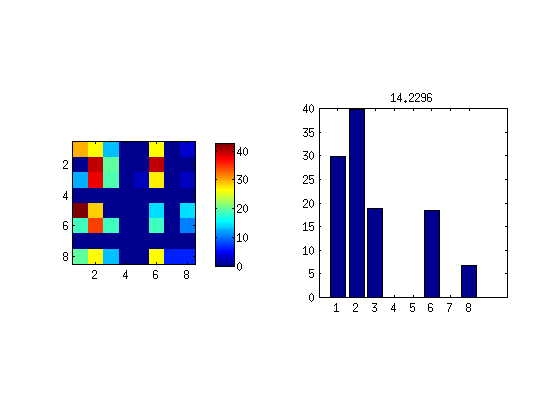
\includegraphics[scale=0.5]{../../../evaluation/feature-sift/fold4_1e5.png}
 \caption{Baseline Fold 4 (top); With SIFT Fold 4 (bottom)}
 \label{figure:withSiftFold4}
\end{figure}

% FOLD 5 RESULTS
\begin{figure}[p]
 \centering
 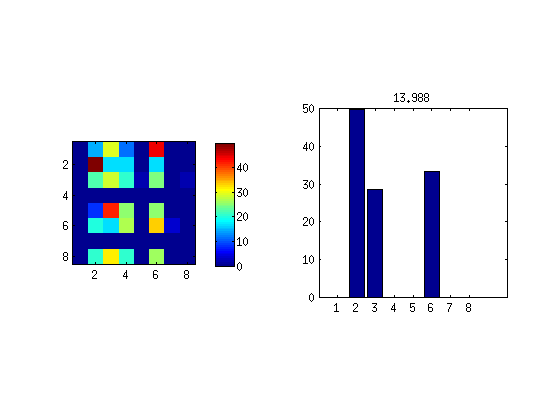
\includegraphics[scale=0.5]{../../../evaluation/baseline/fold5_1e5.png}
 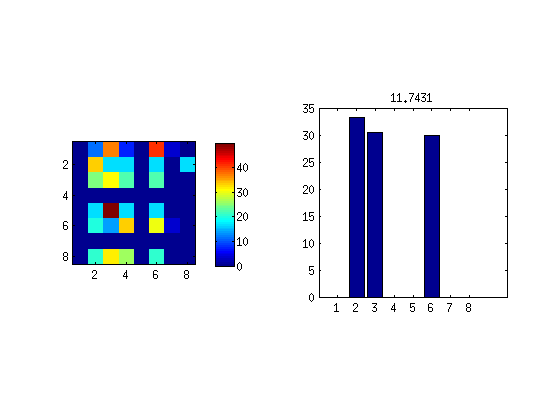
\includegraphics[scale=0.5]{../../../evaluation/feature-sift/fold5_1e5.png}
 \caption{Baseline Fold 5 (top); With SIFT Fold 5 (bottom)}
 \label{figure:withSiftFold5}
\end{figure}


\section{Discussion and Conclusions}

Unfortunately, due to time constraints, the results could not be meaningfully evaluated. From the literature review \cite{luo}, it appears that adding K-Means-clustered SIFT features to the superpixel feature vectors should improve the accuracy of our classifier.

Without data from trials with more superpixels, all we can do is make an educated guess from the literature.

\subsection{Future Work}

Future work should optimize the choice of SVM kernel function, the choice of which features are included in the superpixel feature vectors, and the details of obtaining superpixel SIFT features.

The SVM kernel function could best be a linear, Gaussian, or some degree of polynomial function.  Complete evaluation on the dataset would be the best indicator of the ideal function.  This would be very computationally-intensive, but that would be the hardest part about it.

It is possible that some of the SIFT features included are hurting the accuracy of the classifier. By systematically removing one feature and comparing the accuracy, the bad features could be detected.

As for obtaining the superpixel-level SIFT features, there are many options that were not explored in this project. For one, each superpixel has a small area. This is perhaps not enough for meaningful SIFT features to be extracted. Perhaps, when computing the feature vector for a superpixel, it would be helpful to merge the superpixel with its neighbors for the purpose of computing the SIFT features.  Also, the value of $k$ for the K-Means clustering procedure performed on the SIFT features should be optimized to find the most beneficial value.


{\small
\bibliographystyle{ieee}
\bibliography{egbib}
}

\end{document}
